\documentclass[a4paper, 11pt]{article}
\newcommand\independent{\protect\mathpalette{\protect\independenT}{\perp}}
\def\independenT#1#2{\mathrel{\rlap{$#1#2$}\mkern4mu{#1#2}}}
\usepackage{comment} % enables the use of multi-line comments (\ifx \fi) 
\usepackage{lipsum} %This package just generates Lorem Ipsum filler text. 
\usepackage{fullpage} % changes the margin
\usepackage{tabularx}
\usepackage[a4paper, total={7in, 10in}]{geometry}
\usepackage[fleqn]{amsmath}
\usepackage{amssymb,amsthm}  % assumes amsmath package installed
\newtheorem{theorem}{Theorem}
\newtheorem{corollary}{Corollary}
\usepackage{graphicx}
\usepackage{tikz}
\usetikzlibrary{arrows}
\usepackage{verbatim}
\usepackage[numbered]{mcode}
\usepackage{float}
\usepackage{tikz}
    \usetikzlibrary{shapes,arrows}
    \usetikzlibrary{arrows,calc,positioning}

    \tikzset{
        block/.style = {draw, rectangle,
            minimum height=1cm,
            minimum width=1.5cm},
        input/.style = {coordinate,node distance=1cm},
        output/.style = {coordinate,node distance=4cm},
        arrow/.style={draw, -latex,node distance=2cm},
        pinstyle/.style = {pin edge={latex-, black,node distance=2cm}},
        sum/.style = {draw, circle, node distance=1cm},
    }
\usepackage{xcolor}
\usepackage{mdframed}
\usepackage[shortlabels]{enumitem}
\usepackage{indentfirst}
\usepackage{hyperref}
    
\renewcommand{\thesubsection}{\thesection.\alph{subsection}}

\newenvironment{problem}[2][Problem]
    { \begin{mdframed}[backgroundcolor=gray!20] \textbf{#1 #2} \\}
    {  \end{mdframed}}

% Define solution environment
\newenvironment{solution}
    {\textit{Solution:}}
    {}

\renewcommand{\qed}{\quad\qedsymbol}
%%%%%%%%%%%%%%%%%%%%%%%%%%%%%%%%%%%%%%%%%%%%%%%%%%%%%%%%%%%%%%%%%%%%%%%%%%%%%%%%%%%%%%%%%%%%%%%%%%%%%%%%%%%%%%%%%%%%%%%%%%%%%%%%%%%%%%%%
\begin{document}
%Header-Make sure you update this information!!!!
\noindent
%%%%%%%%%%%%%%%%%%%%%%%%%%%%%%%%%%%%%%%%%%%%%%%%%%%%%%%%%%%%%%%%%%%%%%%%%%%%%%%%%%%%%%%%%%%%%%%%%%%%%%%%%%%%%%%%%%%%%%%%%%%%%%%%%%%%%%%%
\large\textbf{\href{https://linkedin.com/in/Melvin-Mokhtari}{Melvin Mokhtari}} \hfill \textbf{Assignment 3} \\
Email: \href{mailto:melvin.mokhtari@ec.iut.ac.ir}{melvin.mokhtari@ec.iut.ac.ir} \hfill ID: 9831143 \\
\normalsize Course: Artificial Intelligence \hfill Semester: Winter 2023\\
Instructor: {\href{https://samanehoseini.iut.ac.ir/}{Dr. Samaneh Hosseini} \hfill Date: \today \\
%$22^{nd}$ November, 2019
\noindent\rule{7in}{2.8pt}
%%%%%%%%%%%%%%%%%%%%%%%%%%%%%%%%%%%%%%%%%%%%%%%%%%%%%%%%%%%%%%%%%%%%%%%%%%%%%%%%%%%%%%%%%%%%%%%%%%%%%%%%%%%%%%%%%%%%%%%%%%%%%%%%%%%%%%%%
% Problem 1
%%%%%%%%%%%%%%%%%%%%%%%%%%%%%%%%%%%%%%%%%%%%%%%%%%%%%%%%%%%%%%%%%%%%%%%%%%%%%%%%%%%%%%%%%%%%%%%%%%%%%%%%%%%%%%%%%%%%%%%%%%%%%%%%%%%%%%%%
\begin{problem}{1}
%Consider the scalar system
%\begin{align*}
%    \Dot{x} &= -x + u + w
%\end{align*}
%$w$ is zero-mean process noise with a variance of $Q$. The control has a mean value of $u_0$, an uncertainty of $2$ (one standard deviation), and is uncorrelated with $w$. Rewrite the system equations to obtain an equivalent system with a normalized control that is perfectly known. What is the variance of the new process noise term in the transformed system equation?
\end{problem}
%\begin{solution}
%The variance of the new process noise, $w_u$ is $\Sigma_{w_{u}} = Q + \sigma^2_u = Q + 4$.
%\begin{align*}
%    \Dot{x} &= -x + u_0 + \underbrace{w + \Delta u}_{w_{u}}, \quad w_u \sim (0, Q + \sigma^2_u).
%\end{align*}
%\end{solution}
\begin{solution}
	\section*{\small Part 1}
	I'll go over each statement one by one. If a statement is 'true,' it is because of the network structure, and I will also identify the corresponding conditional independence property. If a statement is 'false,' I'll identify the conditional independence assumption required to make it true:
	\begin{itemize}
		\item $P(B, I, M) = P(B)P(I)P(M):$ False, would need $I \independent B \independent M$
		\item $P(J \mid G) = P(J \mid G, I):$ True, $J \independent I \mid G$
		\item $P(M \mid G, B, I) = P(M \mid G, B, I, J):$ True, $M \independent J \mid G, B, I$
	\end{itemize}
	\section*{\small Part 2}
	Let's calculate the value of $P(B, I, M, \neg G, J):$
	\begin{center}
		$P(B, I, M, \neg G, J) = P(J \mid G) \cdot P(G \mid B, I, M, \neg G) \cdot P(B) \cdot P(I \mid B, M) \cdot P(M) \cdot P(\neg G \mid B, I, M) = 0.06561$
\end{center}
\end{solution}  
\noindent\rule{7in}{2.8pt}

%%%%%%%%%%%%%%%%%%%%%%%%%%%%%%%%%%%%%%%%%%%%%%%%%%%%%%%%%%%%%%%%%%%%%%%%%
% Problem 2
%%%%%%%%%%%%%%%%%%%%%%%%%%%%%%%%%%%%%%%%%%%%%%%%%%%%%%%%%%%%%%%%%%%%%%%%%%%%%%%%%%%%%%%%%%%%%%%%%%%%%%%%%%%%%%%%%%%%%%%%%%%%%%%%%%%%%%%%
\pagebreak
\begin{problem}{2}
%Consider the system
%\begin{align*}
%    x_{k+1} &= \phi x_{k} + w_{k}, \\
%    y_k &= x_k, 
%\end{align*}
%where $w_k \sim (0, 1)$, and $\phi = 0.9$ is an unknown constant. Design an extended Kalman filter to estimate $\phi$. Simulate the filter for $100$ time steps with $x_0 = 1, P_0 = I , \hat{x}_{0} = 0$, and $\hat{\phi}_{0} = 0$. Hand in your source code and a plot showing $\hat{\phi}$ as a function of time.
\end{problem}
\begin{solution}
In order to recreate this Bayesian network in such a way that the order of entering the variables is M, B, I, G, and J, we need to assure that the dependencies between the variables are maintained while keeping the desired order.\\
Here's the new structure based on the given order:
\begin{enumerate}
	\item M (no parents)
	\item B (no parents)
	\item I (parents: M, B)
	\item G (parents: I, M, B)
	\item J (parents: G)
\end{enumerate}
So, the new Bayesian network would look like this:
\begin{center}
	\begin{figure}[H]
		\centering
		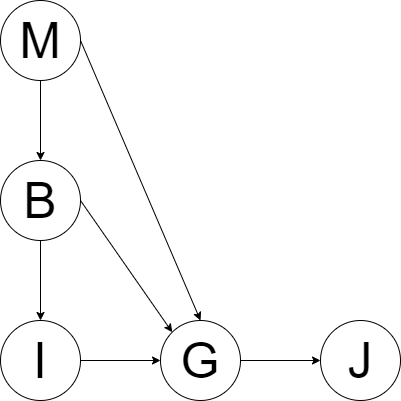
\includegraphics[width=0.4\textwidth]{Untitled Diagram.png}
	\end{figure}
\end{center}
The detailed explanation of the process is as described below:
\begin{enumerate}
	\item Start with the first variable, M, which has no parents. So, M is placed on the rightmost side of the network.
	\item Move to the next variable, B, which also has no parents. Place B to the left of M.
	\item Now, we have I, which has M and B as parents. Place I to the left of B, and create edges from M and B to I.
	\item The next variable is G, which has I, M, and B as parents. Place G to the left of I, and create edges from I, M, and B to G.
	\item Finally, we have J, which has G as its parent. Place J to the left of G, and create an edge from G to J.
\end{enumerate}
\end{solution} 
\noindent\rule{7in}{2.8pt}
%\lstinputlisting{HW6Q2.m}
%\noindent\rule{7in}{2.8pt}
\pagebreak
\begin{problem}{3}

\end{problem}
\begin{solution}
	\begin{itemize}
		\item FALSE; In this Bayesian network, P7 and P3 are not independent of each other because there is a path from P3 to P7 via P4, and P4 is a parent node of P7. Therefore, any changes in P3 or P4 could potentially affect P7.
		\item TRUE; P3 and P2 are dependent on each other, as they share a common child node, P4. Any changes in P4 could potentially affect both P3 and P2.
		\item FALSE; There is no direct or indirect path between P1 and P2, which means they are independent of each other. Changes in one node will not affect the other.
		\item FALSE; P5 and P2 are not independent of each other because there is a path from P2 to P4 to P3 to P5. Therefore, any changes in P2 or P4 could potentially affect P5.
		\item FALSE; P5 and P6 are not independent of each other because there is a path from P5 to P3 to P6. Therefore, any changes in P3 could potentially affect both P5and P6, making them dependent on each other.
	\end{itemize}
\end{solution}
\noindent\rule{7in}{2.8pt}
\pagebreak
%%%%%%%%%%%%%%%%%%%%%%%%%%%%%%%%%%%%%%%%%%%%%%%%%%%%%%%%%%%%%%%%%%%%%%%%%
\begin{problem}{4}
	
\end{problem}
\begin{solution}
	\section*{\small Part 1}
	I'll go over each statement one by one:
	\begin{itemize}
		\item $P(\neg p3) = P(p1)P(p2 \mid p1)P(\neg p3 \mid p2)P(p4 \mid p2) + P(p1)P(p2 \mid p1)P(\neg p3 \mid p2)P(\neg p4 \mid p2) + P(p1)P( \neg p2 \mid p1)P(\neg p3 \mid \neg p2)P(p4 \mid \neg p2) + P(p1)P(\neg p2 \mid p1)P(\neg p3 \mid \neg p2)P(\neg p4 \mid \neg p2) + P(\neg p1)P(p2 \mid \neg p1)P(\neg p3 \mid p2)P(p4 \mid p2) + P(\neg p1)P(p2 \mid \neg p1)P( \neg p3 \mid p2)P(\neg p4 \mid p2) + P(\neg p1)P(\neg p2 \mid \neg p1)P( \neg p3 \mid \neg p2)P(p4 \mid \neg p2) + P(\neg p1)P(\neg p2 \mid \neg p1)P(\neg p3 \mid \neg p2)P(\neg p4 \mid \neg p2) = $
				
		$0.4 \times 0.8 \times 0.8 \times 0.8 + 0.4 \times 0.8 \times 0.8 \times 0.2 + 0.4 \times 0.2 \times 0.7 \times 0.5 + 0.4 \times 0.2 \times 0.7 \times 0.5 + 0.6 \times 0.5 \times 0.8 \times 0.8 + 0.6 \times 0.5 \times 0.8 \times 0.2 + 0.6 \times 0.5 \times 0.7 \times 0.5 + 0.6 \times 0.5 \times 0.7 \times 0.5 = 0.2048 + 0.0512 + 0.028 + 0.028 + 0.192 + 0.048 + 0.105 + 0.105 = \textbf{0.762}$
		\item $P(p2, \neg p3) = P(p1)P(p2 \mid p1)P(\neg p3 \mid p2)P(p4 \mid p2) + P(p1)P(p2 \mid p1)P(\neg p3 \mid p2)P(\neg p4 \mid p2) + P(\neg p1)P(p2 \mid \neg p1)P(\neg p3 \mid p2)P(p4 \mid p2) + P(\neg p1)P(p2 \mid \neg p1)P(\neg p3 \mid p2)P(\neg p4 \mid p2) = $
		
		$0.4 \times 0.8 \times 0.8 \times 0.8 + 0.4 \times 0.8 \times 0.8 \times 0.2 + 0.6 \times 0.5 \times 0.8 \times 0.8 + 0.6 \times 0.5 \times 0.8 \times 0.2 = 0.2048 + 0.0512 + 0.192 + 0.048 = 0.496$\\
		
		$P(p2 \mid \neg p3) =\frac{P(p2, \neg p3)}{P(\neg p3)} = \frac{0.496}{0.762} = \textbf{0.6509}$
		\item $P(p1, p2, \neg p3) = P(p1)P(p2 \mid p1)P(\neg p3 \mid p2)P(p4 \mid p2) + P(p1)P(p2 \mid p1)P(\neg p3 \mid p2)P(\neg p4 \mid p2) = 0.4 \times 0.8 \times 0.8 \times 0.8 + 0.4 \times 0.8 \times 0.8 \times 0.2 = 0.2048 + 0.0512 = 0.256$\\
		
		$P(\neg p1, p2, \neg p3) = P(\neg p1)P(p2 \mid \neg p1)P(\neg p3 \mid p2)P(p4 \mid p2) + P(\neg p1)P(p2 \mid \neg p1)P(\neg p3 \mid p2)P(\neg p4 \mid p2) = 0.6 \times 0.5 \times 0.8 \times 0.8 + 0.6 \times 0.5 \times 0.7 \times 0.2 = 0.192 + 0.048 = 0.24$\\
		
		$P(p2, \neg p3) = P(p1, p2, \neg p3) + P(\neg p1, p , \neg p3) = 0.256 + 0.24 = 0.496$\\
		
		$P(p1 \mid p2, \neg p3) = \frac{P(p1, p2, \neg p3)}{P(p2, \neg p3)} = \frac{0.256}{0.496} = \textbf{0.5161}$
		\item $P(p1, \neg p3, p4) = P(p1)P(p2 \mid p1)P(\neg p3 \mid p2)P(p4 \mid p2) + P(p1)P(\neg p2 \mid p1)P(\neg p3 \mid \neg p2)P(p4 \mid \neg p2) = 0.4 \times 0.8 \times 0.8 \times 0.8 + 0.4 \times 0.2 \times 0.7 \times 0.5 = 0.2048 + 0.028 = 0.2328$\\
		
		$P(\neg p1, \neg p3, p4) = P(\neg p1)P(p2 \mid \neg p1)P(\neg p3 \mid p2)P(p4 \mid p2) + P(\neg p1)P(\neg p2 \mid \neg p1)P(\neg p3 \mid \neg p2)P(p4 \mid \neg p2) = 0.6 \times 0.5 \times 0.8 \times 0.8 + 0.6 \times 0.5 \times 0.7 \times 0.5 = 0.192 + 0.105 = 0.297$\\
		
		$P(\neg p3, p4) = P(p1, \neg p3, p4) + P(\neg p1, \neg p , p4) = 0.2328 + 0.297 = 0.5298$\\
		
		$P(p1 \mid \neg p3, p4) = \frac{P(p1, \neg p3, p4)}{P(\neg p3, p4)} = \frac{0.2328}{0.5298} = \textbf{0.4394}$
	\end{itemize}
	\textbf{In conclusion: $P(\neg p3) = 0.762, P(p2 \mid \neg p3) = 0.6509, P(p1 \mid p2, \neg p3) = 0.5161, P(p1 \mid \neg p3, p4) = 0.4394$}
	\pagebreak
	\section*{\small Part 2}
	We know that variable elimination gradually simplifies the original network by removing hidden variables (those that are neither queries nor evidence). I’ll do this for $P(\neg p3)$ and $P(p2 \mid \neg p3)$.\\
	\begin{figure}[H]
		\centering
		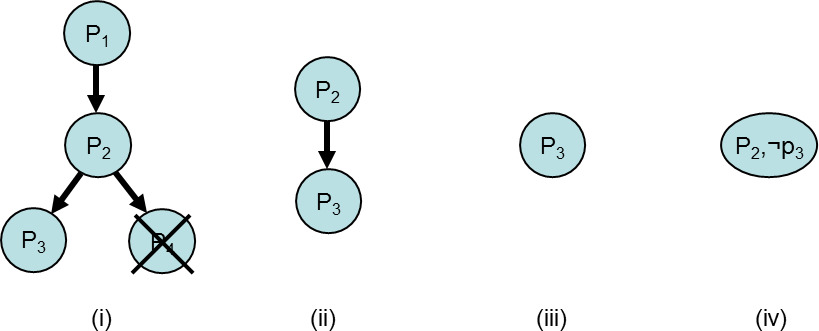
\includegraphics[width=0.72\textwidth]{4-1.jpg}
	\end{figure}
	As shown in the figure above, the first two steps are the same for both probabilities: (i) P4 can simply be removed and (ii) P1 is summed out. Then, (iii) P2 gets summed out to obtain $P(\neg p3)$ while (iv) the particular value $\neg p3$ is taken to obtain $P(p2 \mid \neg p3)$.\\
	The elimination process is carried out by factors. The step (i) is trivial, the step (ii) corresponds to:
	\begin{center}
		$f_{\overline P1}(p2) = 0.4 \times 0.8 + 0.6 \times 0.5 = 0.62$
		
		$f_{\overline P1}(\neg p2) = 0.4 \times 0.2 + 0.6 \times 0.5 = 0.38$
	\end{center}
	The step (iii) consists in:
	\begin{center}
		$f_{\overline P1, \overline P2}(p3) = 0.62 \times 0.2 + 0.38 \times 0.3 = 0.238$
		
		$f_{\overline P1, \overline P2}(\neg p3) = 0.62 \times 0.8 + 0.38 \times 0.7 = 0.762$
	\end{center}
	The step (iv) consists in:
	\begin{center}
		$f_{\overline P1, \neg P3}(p2) = 0.62 \times 0.8 = 0.496$
		
		$f_{\overline P1, \neg P3}(\neg p2) = 0.38 \times 0.7 = 0.266$
	\end{center}
	Eventually, the target probabilities can be computed:
	\begin{center}
		$P(\neg p3) = f_{\overline P1, \overline P2}(\neg p3) = \textbf{0.762}$
		
		$P(p2 \mid \neg p3) = \frac{f_{\overline P1, \neg P3}(p2)}{f_{\overline P1, \neg P3}(p2) + f_{\overline P1, \neg P3}(\neg p2)} = \frac{0.496}{0.496 + 0.266} = \textbf{0.6509}$
	\end{center}
	As expected, variable elimination is frequently "much more efficient" with a proper elimination order (finding the best one is difficult, but heuristics exist). In our example, the enumeration method requires 47 operations, whereas the variable elimination method requires only 16 operations.
\end{solution}
\\\noindent\rule{7in}{2.8pt}
\pagebreak
%%%%%%%%%%%%%%%%%%%%%%%%%%%%%%%%%%%%%%%%%%%%%%%%%%%%%%%%%%%%%%%%%%%%%%%%%
\begin{problem}{5}
	
\end{problem}
\begin{solution}
Let's take a look at them one by one:
\begin{itemize}
	\item $P(Q2 = Happy):$ The question is to find the probability that Mr. X is happy on day 2. It is a given that the first day he was happy. For the second day, we need to find the transition probability $P(Q2 = Happy \mid Q1 = Happy)$, which is equal to 0.8.
	\item We need to calculate the likelihood of an observation frown on day 2. But we don't know if he's happy on day 2 (we know he was on day 1). As a result, the probability of the observation is the product of the observation probabilities and all possible hidden state transitions.\\
	$P(O2 = frown) = P(O1 = frown) = P(O2 = frown \mid Q2 = Happy) + P(O2 = frown \mid Q2 = Angry) = P(Happy \mid Happy) \times P(frown \mid Happy) + P(Angry \mid Happy) \times P(frown \mid Angry) = (0.8 \mid 0.1) + (0.2 \mid 0.5) = 0.08 + 0.1 = 0.18$
	\item $P(Q2 = Happy \mid O2 = frown) = \frac{P(O2 = frown \mid Q2 = Happy) P(Q2 = Happy)}{P(O2 = frown)} = \frac{4}{9}$\\
	$P(Q2 = Happy \mid O1 = frown) = \frac{P(O1 = frown \mid Q2 = Happy) P(Q2 = Happy)}{P(O1 = frown)} = \frac{4}{9}$\\
	$P(Q2 \mid O2 = \text{frown}, O1 = \text{frown}) =$\\
	$\frac{{P(O2 = \text{frown} \mid Q2 = \text{Happy}) \cdot P(O1 = \text{frown} \mid Q2 = \text{Happy}) \cdot P(Q2 = \text{Happy})}}{{P(O2 = \text{frown}, O1 = \text{frown} \mid Q2 = \text{Happy}) \cdot P(Q2 = \text{Happy}) + P(O2 = \text{frown}, O1 = \text{frown} \mid Q2 = \text{Angry}) \cdot P(Q2 = \text{Angry})}}
	$
\end{itemize} 
\end{solution}
\noindent\rule{7in}{2.8pt}
\pagebreak
%%%%%%%%%%%%%%%%%%%%%%%%%%%%%%%%%%%%%%%%%%%%%%%%%%%%%%%%%%%%%%%%%%%%%%%%%
\begin{problem}{6}
	
\end{problem}
\begin{solution}
For all values of t, the filtering formula is:
\begin{figure}[H]
	\centering
	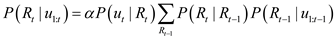
\includegraphics[width=0.5\textwidth]{6-1.png}
\end{figure}
At the fixed point, it is expected that:
\begin{figure}[H]
	\centering
	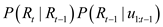
\includegraphics[width=0.25\textwidth]{6-2.png}
\end{figure}
Assume the fixed-point probability is <$p , 1-p$>. This produces the following equations:
\begin{figure}[H]
	\centering
	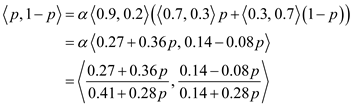
\includegraphics[width=0.52\textwidth]{6-3.png}
\end{figure}
From the penultimate equality $\alpha = \frac{1}{0.41 + 0.28p}.$ So:
\begin{figure}[H]
	\centering
	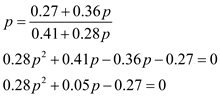
\includegraphics[width=0.32\textwidth]{6-4.png}
\end{figure}
Then the two roots of the above quadratic equation are $p=0.8967, -1.0753$. The positive root will determine the values for the fixed point which is <$0.8967 , 0.1033$>.\\ \\
It is given that the probability of rain on day 0 is $P(R_0) = $ <$0.5 , 0.5$>and same is the probability of rain on day 1. \\ \\
Here, the computed probability is \textbf{<$\textbf{0.8967 , 0.1033}$>}, indicating that as the days pass, the probability of rain on the current day increases monotonically toward a fixed point.
\end{solution}
\\\noindent\rule{7in}{2.8pt}
\pagebreak
%%%%%%%%%%%%%%%%%%%%%%%%%%%%%%%%%%%%%%%%%%%%%%%%%%%%%%%%%%%%%%%%%%%%%%%%%
\end{document}
 